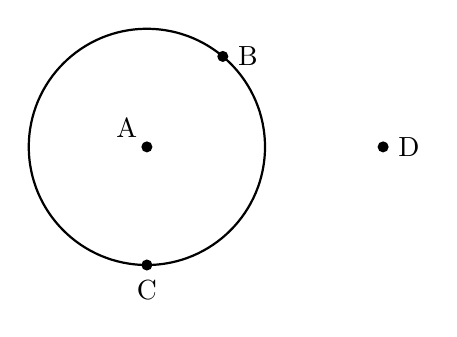
\begin{tikzpicture}[scale=1]

    % Define the center point A
    \coordinate (A) at (0,0);
    
    % Define the radius of the circle
    \def\R{1.5}

    % Draw the main circle
    \draw[thick] (A) circle (\R);

    % Draw the dot for the center point A
    \fill (A) circle (2pt);
    % Label A placed slightly above and to the left of the center dot
    \node[above left] at (A) {A};

    % Define and draw point B on the circle (approximately at 50 degrees)
    \coordinate (B) at (50:\R);
    \fill (B) circle (2pt);
    % Label B placed to the right of point B
    \node[right, xshift=2pt] at (B) {B};

    % Define and draw point C at the bottom of the circle (270 degrees)
    \coordinate (C) at (270:\R);
    \fill (C) circle (2pt);
    % Label C placed below point C
    \node[below, yshift=-2pt] at (C) {C};

    % Define and draw point D outside the circle, horizontally to the right
    \coordinate (D) at (3, 0);
    \fill (D) circle (2pt);
    % Label D placed to the right of point D
    \node[right, xshift=2pt] at (D) {D};

\end{tikzpicture}